\documentclass{article}
\usepackage[utf8]{inputenc}
\usepackage{float}

\title{ECS 145 Term Project}
\author{Gavin Grey, Jeremy Kwan, Shayan Mandegarian, Michael Nguyen}
\date{}

\usepackage{natbib}
\usepackage{graphicx}

\begin{document}

\maketitle

\section{Introduction}
For our term project, we had to write a function of call form exploreShape(x, estMethod, tuning, twoAtATime) where x is a numeric vector, estMethod is whether we want to graph a histogram or a density graph, tuning is the number of breaks for a histogram, or the bw value of the density graph, and twoAtATime is whether we want to superimpose the previous graph onto a new graph.


\section{Graphing}

\begin{figure}[H]
\centering
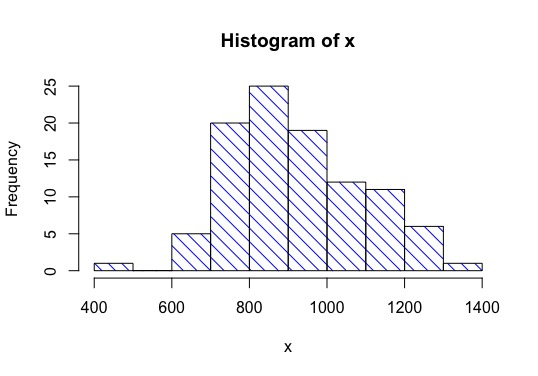
\includegraphics[scale=0.5]{Nile, 7 histogram.jpeg}
\caption{Sample output explore(Nile, 'hist', 7, T)}
\label{fig:Nile histogram 7}
\end{figure}


\begin{figure}[H]
\centering
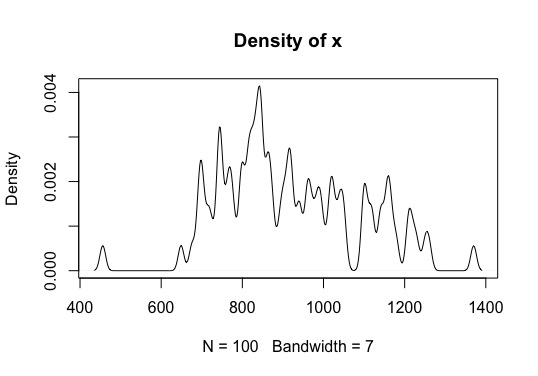
\includegraphics[scale=0.5]{Nile, 7 Tuning param.jpeg}
\caption{Sample output explore(Nile, 'density', 7, T)}
\label{fig:Nile density graph 7}
\end{figure}


\subsection{Changing Tuning Parameter}
Whenever we change the tuning parameter of the graph, if twoAtATime is initialized as true, then the previous graph is kept and superimposed onto the other graph. The previous graph is colored red to help differentiate between the graphs. To do this, we use a global variable that keeps track of the previous tuning parameter, so that when we graph with some new parameter, the old graph can be superimposed on top of it, and the new parameter gets stored into the global variable.

\begin{figure}[H]
\centering
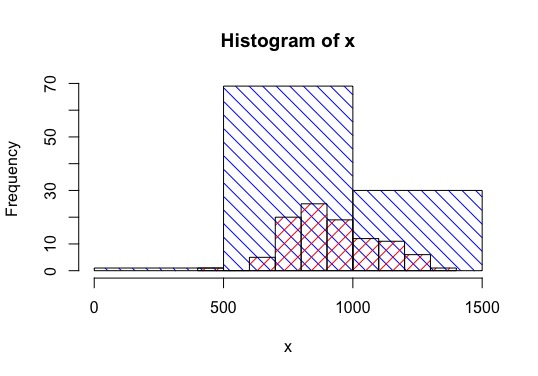
\includegraphics[scale=0.5]{Nile, 3 superimposed on 7 hist.jpeg}
\caption{Sample output explore(Nile, 'hist', 7, T), then changed tuning parameter to 3.}
\label{fig:Nile histogram 3 on 7}
\end{figure}

\begin{figure}[H]
\centering
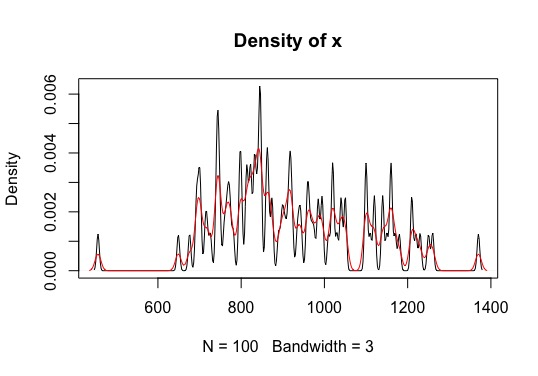
\includegraphics[scale=0.5]{Nile, 7 superimposed on 3.jpeg}
\caption{Sample output explore(Nile, 'density', 7, T) and then changed tuning parameter to 3. }
\label{fig:Nile density graph 3 on 7}
\end{figure}

\subsection{Animation}
To implement animations, we simply looped through multiple different tuning parameters, starting from 1 and stopping at 100. At each tuning parameter, the data is plotted and then the tuning parameter is incremented. This animation will not superimpose, even if the user specified to superimpose the other plots.

\subsection{Zooming In and Out}
Additionally, we included zooming functionality. This was done by first ordering the data set, then removing the first 10 and the last 10 points of data, in the case of zooming in. Then in the case of zooming out, we restore the original data set. To do this we keep the original data set stored in a global variable that is set any time we pass a new data set to our function.

\begin{figure}[H]
\centering
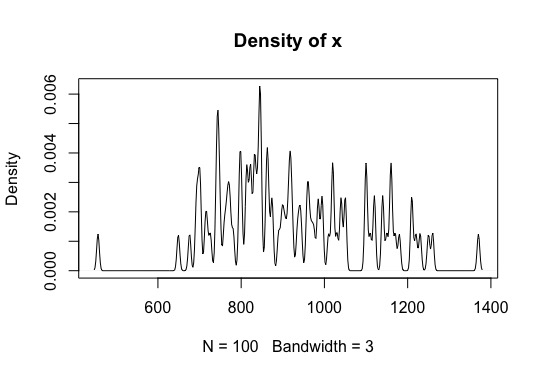
\includegraphics[scale=0.5]{Nile, 3 density before zoom.jpeg}
\caption{Sample output explore(Nile, 'density', 3, F) }
\label{fig:Nile density graph 3}
\end{figure}


\begin{figure}[H]
\centering
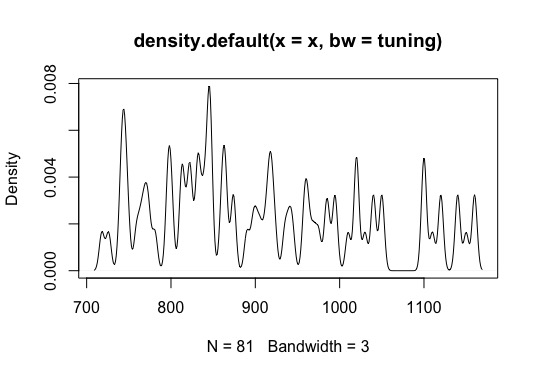
\includegraphics[scale=0.5]{Nile, 3 density after zoom in.jpeg}
\caption{Sample output explore(Nile, 'density', 3, F) zoomed in. }
\label{fig:Nile density graph 3, zoom in}
\end{figure}




\section{Individual Contributions}

\subsection{Gavin}
Gavin worked on debugging the code when errors arose, as well as brainstorming the implementation of various aspects of the code and writing the Graphing section of the report.

\subsection{Jeremy}
Initially the code was run automatically with the file, and not with a function call to exploreShape, but Jeremy put the code within the exploreShape function such that the loop and prompts went within that itself. Thus, the graphing occurred only when the user prompts it with the function exploreShape with the correct arguments. Jeremy helped with testing of the project code, and pointing out issues in output. Furthermore, Jeremy helped with outlining and organization of the report, writing the introduction as well as adding in the images of output graphs.

\subsection{Shayan}

\subsection{Michael}

%\section{Conclusion}
%``I always thought something was fundamentally wrong with the universe'' %\citep{adams1995hitchhiker}

%\bibliographystyle{plain}
%\bibliography{references}

\end{document}
